\documentclass[11pt,a4paper]{article}
\usepackage[a4paper,top=2.2cm,bottom=2.4cm,left=2.2cm,right=2.2cm]{geometry}
\usepackage{mathptmx}
\usepackage[T1]{fontenc}
\usepackage{graphicx}
\usepackage{xcolor}
\usepackage{fancyhdr}
\usepackage{tikz}
\usetikzlibrary{positioning,arrows.meta,shapes.geometric,fit,backgrounds,calc}
\usepackage{array,tabularx}
\usepackage{enumitem}
\usepackage[breakable]{tcolorbox}
\usepackage{xurl}
\usepackage[hidelinks]{hyperref}

% ---------------- EDIT THESE ----------------
\newcommand{\coursename}{COURSE NAME AND ID}   % e.g. "DATA STRUCTURES (TCS-302)"
\newcommand{\teamname}{[Team Name] \quad Team \# [No.]}
% Put geulogo.png, member1.png ... member4.png next to this file and recompile.
% --------------------------------------------

\definecolor{banner}{RGB}{0,103,152}
\definecolor{bannertext}{RGB}{255,204,41}
\definecolor{subhead}{RGB}{46,90,150}
\definecolor{hint}{RGB}{130,130,130}

\pagestyle{fancy}
\fancyhf{}
\lhead{\small\coursename}
\rhead{\small PHASE-III PROJECT PROGRESS}
\rfoot{\small Page \thepage}
\renewcommand{\headrulewidth}{0pt}
\AddToHook{shipout/background}{%
  \begin{tikzpicture}[remember picture,overlay]
    \fill[bannertext] (current page.south west) rectangle ([yshift=0.18cm]current page.south east);
  \end{tikzpicture}}

\setlength{\parindent}{0pt}
\setlength{\parskip}{3pt}
\setlist{nosep,leftmargin=1.2em}

\newcommand{\banner}[1]{\vspace{6pt}\noindent\colorbox{banner}{\parbox{\dimexpr\linewidth-2\fboxsep}{\vspace{4pt}\Large\bfseries\color{bannertext}#1\vspace{4pt}}}\vspace{8pt}}
\newcommand{\qhead}[2]{\vspace{8pt}{\color{subhead}\LARGE #1}\\[-1pt]{\color{hint}\small #2}\par\vspace{2pt}}
\newtcolorbox{answer}{colback=white,colframe=black,boxrule=0.6pt,before skip=4pt,after skip=6pt,arc=0pt,left=6pt,right=6pt,top=4pt,bottom=4pt,fontupper=\small}
\newcommand{\img}[2]{\IfFileExists{#1}{\includegraphics[height=#2]{#1}}{\fbox{\parbox[c][#2][c]{#2}{\centering\scriptsize\texttt{#1}}}}}

\begin{document}

% ================= PAGE 1 =================
\IfFileExists{geulogo.jpg}{\includegraphics[width=9cm]{geulogo.jpg}}{\img{geulogo.png}{6cm}}

\banner{PROJECT AND TEAM INFORMATION}

\qhead{Project Title}{(Try to choose a catchy title. Max 20 words).}
\begin{answer}
\textbf{SmartWaste: Priority-Driven Smart Garbage Collection and Route Optimization}
\end{answer}

\newpage
% ================= PAGE 2 =================
\renewcommand{\arraystretch}{1.25}
\begin{tabularx}{\dimexpr\linewidth-2pt}{|X|>{\raggedright\arraybackslash}p{5.6cm}|}
\hline
\textit{Team Name:}\newline\textit{Team \#} & \textit{\teamname} \\ \hline
\textbf{Team member 1 (Team Lead)}\newline\textit{(Last Name, name: student ID: email, picture):} &
\textit{Singh
Manthan}\newline\textit{2510350070}\newline\textit{smanthan236@gmail.com}\newline\img{member1.jpg}{2.2cm} \\ \hline
\textbf{Team member 2}\newline\textit{(Last Name, name: student ID: email, picture):} &
\textit{Singh
Shaurya Pratap}\newline\textit{2510011689}\newline{\footnotesize\textit{shauryapratpsinghtomar18@gmail.com}}\newline\img{member2.png}{2.2cm} \\ \hline
\textbf{Team member 3}\newline\textit{(Last Name, name: student ID: email, picture):} &
\textit{Rana
Aryan}\newline\textit{2510350073}\newline\textit{aryanrana811@gmail.com}\newline\img{member3.jpg}{2.2cm} \\ \hline
\textbf{Team member 4}\newline\textit{(Last Name, name: student ID: email, picture):} &
\textit{Hritambra}\newline\textit{2510380105}\newline\textit{riturawat442@gmail.com}\newline\img{member4.jpg}{2.2cm} \\ \hline
\end{tabularx}

\newpage
% ================= PAGE 3 =================
\banner{PHASE-III PROJECT PROGRESS DESCRIPTION (35 pts)}

\qhead{Project Abstract (2 pts)}{(Brief restatement of your project's main goal. Max 300 words).}
\begin{answer}
Most municipal garbage collection runs on fixed routes and fixed schedules, regardless of how full each bin actually is. Busy locations overflow before the truck arrives, while trucks waste fuel and time visiting bins that are nearly empty. \textbf{SmartWaste} replaces this static model with a data-driven, priority-based one.
\par\medskip
Every bin is stored with its location node, capacity and current fill percentage, and the city road network is modelled as a weighted, undirected graph. A \textbf{max-heap} orders bins by fill level so the most urgent bins are serviced first. For each selected bin, \textbf{Dijkstra's shortest-path algorithm} finds the nearest available truck that still has enough spare capacity, and the assignment is saved to an SQLite database. When a truck's load reaches 90\% of its capacity it is marked \emph{NeedsDepot} and routed to the nearest depot to unload, after which it becomes available again.
\par\medskip
The algorithmic core (written in C) is wrapped in an object-oriented C++ backend that exposes a REST API, with role-based authentication. Three web portals sit on top of it: an \textbf{Admin} portal (bins, trucks, drivers, complaints, reports), a \textbf{Driver} portal (assigned work and truck status) and a \textbf{Citizen} portal (register, raise complaints, track their status). The project aims to cut overflow risk and unnecessary travel compared with fixed-route collection, and to show core data structures and algorithms working inside a complete, usable system.
\end{answer}

\qhead{Updated Project Approach and Architecture (2 pts)}{(Describe your current approach, including system design, communication protocols, libraries used, etc. Max 300 words).}
\begin{answer}
SmartWaste uses a \textbf{three-layer architecture}:\par\smallskip
\textbf{1. DSA core (C, \texttt{dsa/}).} \texttt{graph.c} stores the road network as an adjacency list (undirected, weighted in km). \texttt{heap.c} is an array-based max-heap keyed on fill percentage ($O(\log n)$ insert/extract). \texttt{dijkstra.c} computes shortest paths ($O(V^2)$), reconstructs the full route and guards against integer overflow during relaxation.
\par\medskip
\textbf{2. Backend (C++, \texttt{backend/}).} The domain classes \texttt{Bin}, \texttt{Truck}, \texttt{Driver} and \texttt{Depot} model the entities. \texttt{CollectionManager} calls the C modules through \texttt{extern "C"} and runs the workflow: \emph{load data $\rightarrow$ build heap $\rightarrow$ pick nearest eligible truck $\rightarrow$ record assignment $\rightarrow$ complete collection $\rightarrow$ return to depot when $\geq$90\% full}. \texttt{Database} wraps \textbf{SQLite3} (tables: bins, trucks, drivers, depots, assignments, complaints, collection\_history, gps\_locations). Every change is written to the database first, and only then to the in-memory objects. \texttt{AuthManager} handles salted password hashing (\textbf{OpenSSL}), session tokens, role checks (admin/driver/citizen), driver sign-up approval by the admin, and citizen profile updates.
\par\medskip
\textbf{3. Communication and frontend.} \texttt{api.cpp} and \texttt{authapi.cpp} expose REST endpoints over HTTP using \textbf{cpp-httplib}, with JSON request and response bodies handled by \textbf{nlohmann/json}. The portals (\texttt{frontend/admin}, \texttt{driver}, \texttt{citizen}) are plain HTML, CSS and JavaScript. They call the API with \texttt{fetch} and send the session token with each request.
\par\medskip
\textbf{Design choices.} We kept the algorithms in C so the DSA logic stays explicit and testable on its own, and used C++ OOP for the domain model. SQLite was chosen because it needs no server and still persists state across restarts (active assignments are reloaded at startup). Figure~1 shows the architecture and Figure~2 the end-to-end collection workflow.
\end{answer}

\newpage
{\color{subhead}\large\textbf{Figure 1 -- System Architecture}}\par\vspace{6pt}
\noindent\resizebox{\linewidth}{!}{%
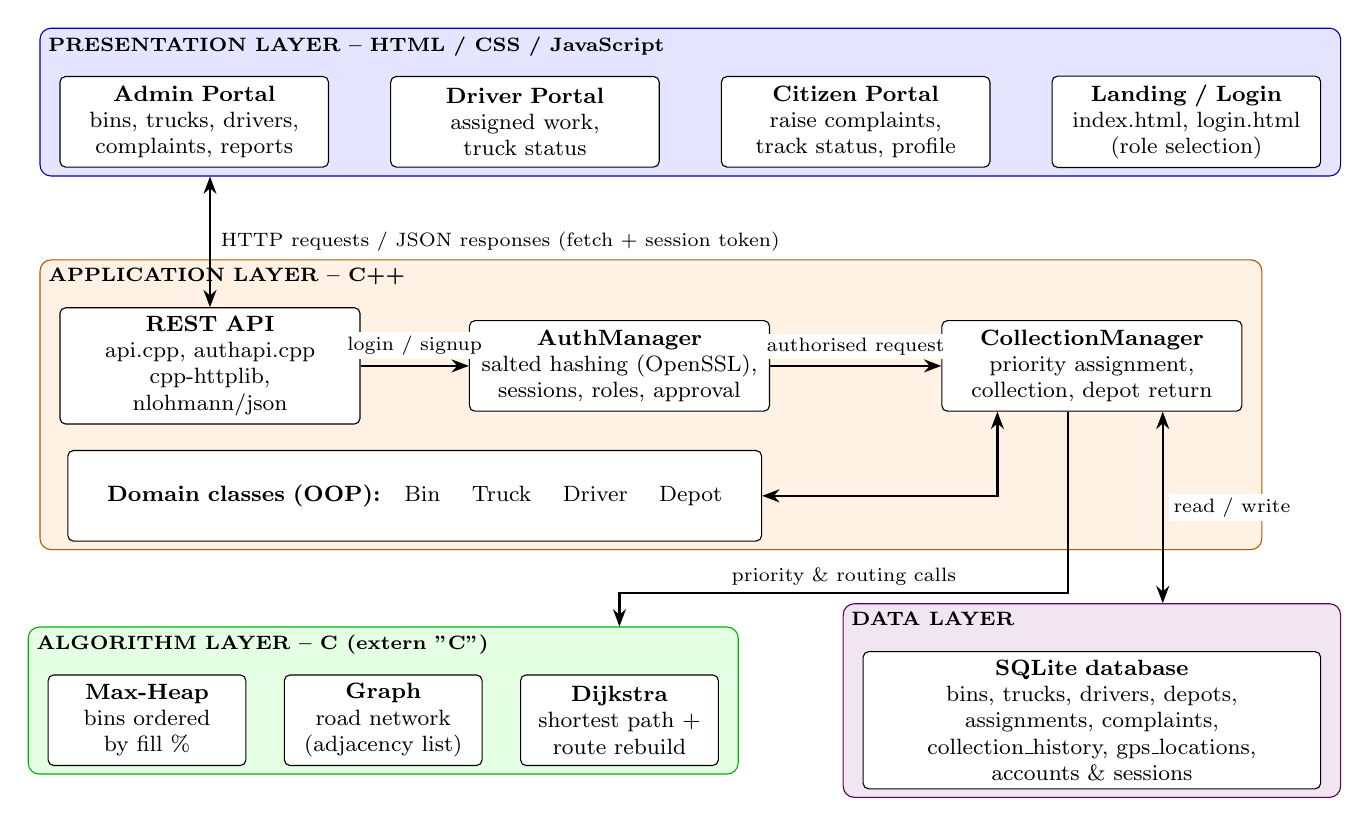
\begin{tikzpicture}[
  font=\footnotesize,
  box/.style={draw, rounded corners=2pt, fill=white, align=center, minimum height=1.15cm, text width=#1, inner sep=3pt},
  box/.default=3.2cm,
  layer/.style={draw=#1!70!black, fill=#1!10, rounded corners=4pt, inner sep=7pt},
  lbl/.style={font=\scriptsize\bfseries, anchor=north west, inner sep=3pt},
  arr/.style={-{Stealth[length=2.2mm]}, thick},
  darr/.style={{Stealth[length=2.2mm]}-{Stealth[length=2.2mm]}, thick},
  tag/.style={font=\scriptsize, fill=white, inner sep=1.5pt}
]
% ---- Presentation layer
\node[box] (admin)   at (0,0)    {\textbf{Admin Portal}\\ bins, trucks, drivers,\\ complaints, reports};
\node[box] (driver)  at (4.2,0)  {\textbf{Driver Portal}\\ assigned work,\\ truck status};
\node[box] (citizen) at (8.4,0)  {\textbf{Citizen Portal}\\ raise complaints,\\ track status, profile};
\node[box] (login)   at (12.6,0) {\textbf{Landing / Login}\\ index.html, login.html\\ (role selection)};
\begin{scope}[on background layer]
  \node[layer=blue, fit=(admin)(login), yshift=2.5mm, inner ysep=10pt] (L1) {};
\end{scope}
\node[lbl] at (L1.north west) {PRESENTATION LAYER -- HTML / CSS / JavaScript};

% ---- Application layer
\node[box=3.6cm] (api)  at (0.2,-3.1)  {\textbf{REST API}\\ api.cpp, authapi.cpp\\ cpp-httplib, nlohmann/json};
\node[box=3.6cm] (auth) at (5.4,-3.1)  {\textbf{AuthManager}\\ salted hashing (OpenSSL),\\ sessions, roles, approval};
\node[box=3.6cm] (cm)   at (11.4,-3.1) {\textbf{CollectionManager}\\ priority assignment,\\ collection, depot return};
\node[box=8.6cm] (dom)  at (2.8,-4.75) {\textbf{Domain classes (OOP):}\quad Bin \quad Truck \quad Driver \quad Depot};
\begin{scope}[on background layer]
  \node[layer=orange, fit=(api)(cm)(dom), yshift=2.5mm, inner ysep=10pt] (L2) {};
\end{scope}
\node[lbl] at (L2.north west) {APPLICATION LAYER -- C++};

% ---- Algorithm layer
\node[box=2.3cm] (heap)  at (-0.6,-7.6) {\textbf{Max-Heap}\\ bins ordered\\ by fill \%};
\node[box=2.3cm] (graph) at (2.4,-7.6)  {\textbf{Graph}\\ road network\\ (adjacency list)};
\node[box=2.3cm] (dij)   at (5.4,-7.6)  {\textbf{Dijkstra}\\ shortest path +\\ route rebuild};
\begin{scope}[on background layer]
  \node[layer=green, fit=(heap)(dij), yshift=2.5mm, inner ysep=10pt] (L3) {};
\end{scope}
\node[lbl] at (L3.north west) {ALGORITHM LAYER -- C (extern "C")};

% ---- Data layer
\node[box=5.6cm] (db) at (11.4,-7.6) {\textbf{SQLite database}\\ bins, trucks, drivers, depots,\\ assignments, complaints,\\ collection\_history, gps\_locations,\\ accounts \& sessions};
\begin{scope}[on background layer]
  \node[layer=violet, fit=(db), yshift=2.5mm, inner ysep=10pt] (L4) {};
\end{scope}
\node[lbl] at (L4.north west) {DATA LAYER};

% ---- Arrows
\draw[darr] (api.north |- L1.south) -- node[tag, right=2pt]{HTTP requests / JSON responses (fetch + session token)} (api.north);
\draw[arr] (api) -- node[tag, above=2pt]{login / signup} (auth);
\draw[arr] (auth) -- node[tag, above=2pt]{authorised request} (cm);
\draw[darr] ([xshift=-1.2cm]cm.south) |- (dom.east);
\draw[arr] ([xshift=-0.3cm]cm.south) -- ++(0,-2.3) -| node[tag, pos=0.25, above=1pt]{priority \& routing calls} (dij.north |- L3.north);
\draw[darr] ([xshift=0.9cm]cm.south) -- node[tag, right=2pt]{read / write} ([xshift=0.9cm]cm.south |- L4.north);
\end{tikzpicture}}

\vspace{14pt}
{\color{subhead}\large\textbf{Figure 2 -- Collection Workflow}}\par\vspace{6pt}
\noindent\resizebox{\linewidth}{!}{%
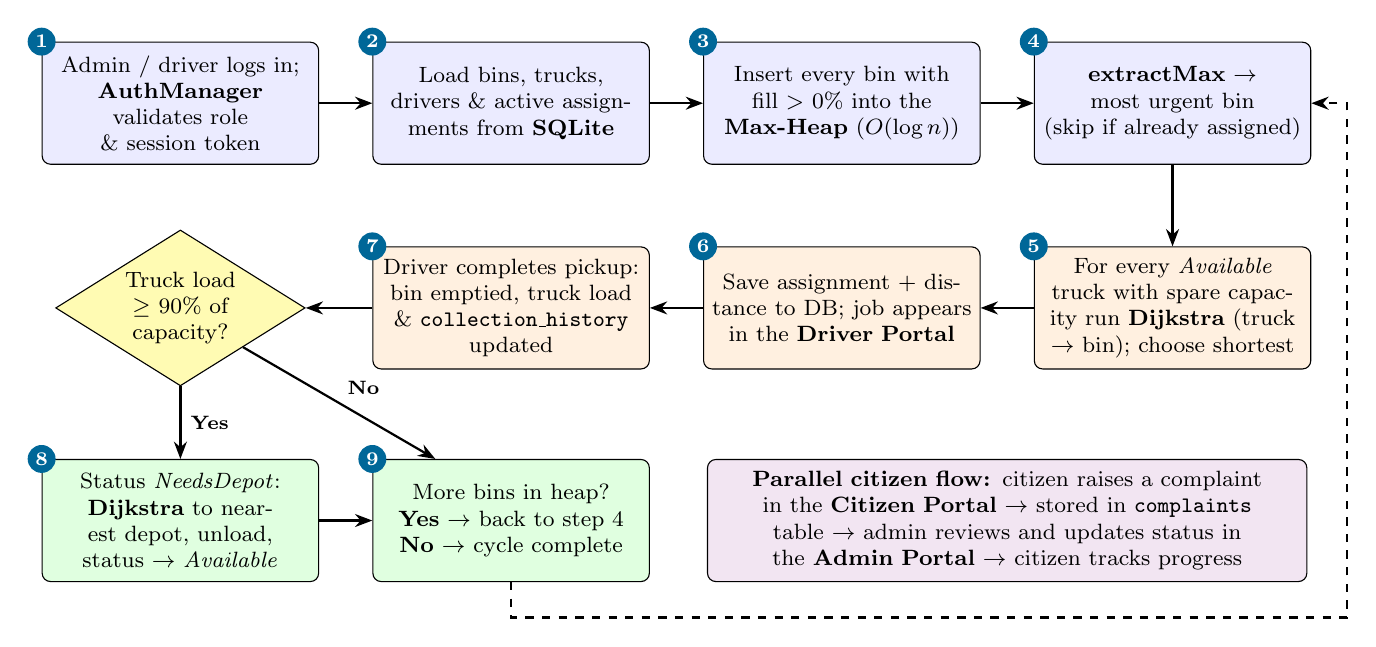
\begin{tikzpicture}[
  font=\footnotesize,
  step/.style={draw, rounded corners=3pt, fill=#1, align=center, text width=3.3cm, minimum height=1.55cm, inner sep=3pt},
  step/.default=blue!8,
  dec/.style={draw, diamond, aspect=1.6, fill=yellow!30, align=center, inner sep=0pt, text width=1.7cm},
  arr/.style={-{Stealth[length=2.2mm]}, thick},
  num/.style={circle, fill=banner, text=white, font=\scriptsize\bfseries, inner sep=1.3pt},
  tag/.style={font=\scriptsize\bfseries}
]
% Row 1 (left -> right)
\node[step] (s1) at (0,0)    {Admin / driver logs in;\\ \textbf{AuthManager} validates role \& session token};
\node[step] (s2) at (4.2,0)  {Load bins, trucks, drivers \& active assignments from \textbf{SQLite}};
\node[step] (s3) at (8.4,0)  {Insert every bin with fill $>$ 0\% into the \textbf{Max-Heap} ($O(\log n)$)};
\node[step] (s4) at (12.6,0) {\textbf{extractMax} $\rightarrow$ most urgent bin\\ (skip if already assigned)};
% Row 2 (right -> left)
\node[step=orange!12] (s5) at (12.6,-2.6) {For every \emph{Available} truck with spare capacity run \textbf{Dijkstra} (truck $\rightarrow$ bin); choose shortest};
\node[step=orange!12] (s6) at (8.4,-2.6)  {Save assignment + distance to DB; job appears in the \textbf{Driver Portal}};
\node[step=orange!12] (s7) at (4.2,-2.6)  {Driver completes pickup: bin emptied, truck load \& \texttt{collection\_history} updated};
\node[dec] (d1) at (0,-2.6) {Truck load\\ $\geq$ 90\% of\\ capacity?};
% Row 3
\node[step=green!12] (s8) at (0,-5.3)   {Status \emph{NeedsDepot}: \textbf{Dijkstra} to nearest depot, unload, status $\rightarrow$ \emph{Available}};
\node[step=green!12] (s9) at (4.2,-5.3) {More bins in heap?\\ \textbf{Yes} $\rightarrow$ back to step 4\\ \textbf{No} $\rightarrow$ cycle complete};
\node[step=violet!10, text width=7.4cm] (c1) at (10.5,-5.3) {\textbf{Parallel citizen flow:} citizen raises a complaint in the \textbf{Citizen Portal} $\rightarrow$ stored in \texttt{complaints} table $\rightarrow$ admin reviews and updates status in the \textbf{Admin Portal} $\rightarrow$ citizen tracks progress};

\foreach \n/\k in {s1/1,s2/2,s3/3,s4/4,s5/5,s6/6,s7/7,s8/8,s9/9}{\node[num] at (\n.north west) {\k};}

\draw[arr] (s1) -- (s2);
\draw[arr] (s2) -- (s3);
\draw[arr] (s3) -- (s4);
\draw[arr] (s4) -- (s5);
\draw[arr] (s5) -- (s6);
\draw[arr] (s6) -- (s7);
\draw[arr] (s7) -- (d1);
\draw[arr] (d1) -- node[tag, right]{Yes} (s8);
\draw[arr] (d1.south east) -- node[tag, above right=-1pt]{No} ([xshift=8mm]s9.north west);
\draw[arr] (s8) -- (s9);
\draw[arr, dashed] (s9.south) -- ++(0,-0.45) -| ([xshift=0.45cm]s5.east |- s4.east) -- (s4.east);
\end{tikzpicture}}


\newpage
% ================= PAGE 4 =================
\qhead{Tasks Completed (7 pts)}{(Describe the main tasks that have been assigned and already completed. Max 250 words).}
{\small
\renewcommand{\arraystretch}{1.2}
\begin{tabularx}{\linewidth}{|X|p{4.6cm}|}
\hline
\textbf{Task Completed} & \textbf{Team Member} \\ \hline
Max-heap priority queue for bin urgency, with unit test (\texttt{heap.c}) & Hritambra \\ \hline
Road-network graph (adjacency list) and Dijkstra shortest path with route reconstruction, plus tests & Hritambra \\ \hline
OOP domain classes \texttt{Bin}, \texttt{Truck}, \texttt{Driver}, \texttt{Depot} & Aryan Rana \\ \hline
\texttt{CollectionManager}: priority assignment, collection completion, return to nearest depot (C/C++ integration) & Aryan Rana, Hritambra \\ \hline
Authentication: salted hashing, sessions, roles, driver approval, \texttt{create\_admin} utility & Aryan Rana \\ \hline
Database schema design (\texttt{schema.sql}, \texttt{auth\_schema.sql}) & Shaurya Pratap Singh \\ \hline
SQLite \texttt{Database} layer (load/save, assignments, collection history) and \texttt{database\_test.cpp} & Shaurya Pratap Singh \\ \hline
REST API endpoints (\texttt{api.cpp}, \texttt{authapi.cpp}) and backend--frontend integration & Manthan Singh, Aryan Rana \\ \hline
Landing page and login/registration page (\texttt{index.html}, \texttt{login.html}) & Manthan Singh \\ \hline
Admin portal: dashboard, bins, trucks, drivers, complaints, reports & Manthan Singh \\ \hline
Driver portal: dashboard, assigned work, truck status & Shaurya Pratap Singh \\ \hline
Citizen portal: complaint submission, status tracking, profile management & Shaurya Pratap Singh \\ \hline
Portal styling and responsive UI (CSS for all portals) & Shaurya Pratap Singh \\ \hline
Testing and validation (unit, integration, end-to-end) & All members \\ \hline
Repository setup, README, documentation and progress report & Manthan Singh \\ \hline
\end{tabularx}}

\qhead{Challenges/Roadblocks (7 pts)}{(Describe the challenges that you have faced or are facing so far and how you plan to solve them. Max 300 words).}
\begin{answer}
All of the challenges below came up during development and have been resolved.\par\smallskip
\textbf{1.} \textbf{Mixing C and C++.} The C modules use fixed-size structs (\texttt{char binID[10]}, \texttt{MAX\_BINS}, \texttt{MAX\_NODES}), while the backend uses C++ strings and vectors. \emph{Solution:} we linked the two through \texttt{extern "C"} headers, converted IDs with bounded \texttt{snprintf}, and kept array limits consistent between the two layers.
\par\medskip
\textbf{2.} \textbf{Keeping memory and database in sync.} If a step failed partway, the in-memory objects and SQLite could disagree. \emph{Solution:} every change is written to the database first and only then applied to the objects, and active assignments are reloaded from the database when the server starts.
\par\medskip
\textbf{3.} \textbf{Choosing the right truck.} Picking the closest truck is not enough, because it might be busy or already full. \emph{Solution:} a truck is considered only if its status is \emph{Available} and it has enough spare capacity. Dijkstra is then run from each such truck, and the shortest real road distance wins.
\par\medskip
\textbf{4.} \textbf{Trucks filling up.} A truck could keep accepting bins after it was nearly full. \emph{Solution:} once a truck's load reaches 90\% of capacity it is marked \emph{NeedsDepot}, routed to the nearest depot by Dijkstra, unloaded, and set back to Available.
\par\medskip
\textbf{5.} \textbf{Secure multi-role access.} Admins, drivers and citizens need different permissions. \emph{Solution:} salted password hashing with OpenSSL, session tokens checked on every request, role validation, and admin approval before a new driver account becomes active.
\par\medskip
\textbf{6.} \textbf{Setup and data hygiene.} Building with OpenSSL and cpp-httplib on Windows took effort, and the local database file must not be committed. \emph{Solution:} we documented the dependencies and added the SQLite file to \texttt{.gitignore}.
\end{answer}

\newpage
\qhead{Project Outcome/Deliverables (2 pts)}{(Describe what are the key outcomes / deliverables of the project. Max 200 words).}
\begin{answer}
\begin{itemize}
\item A reusable C library of data structures and algorithms (graph, max-heap, Dijkstra), with unit tests.
\item A C++ backend: the domain model, the collection-optimization engine and a REST API server.
\item A persistent SQLite database (bins, trucks, drivers, depots, assignments, complaints, collection history, GPS locations).
\item Secure, role-based authentication for admins, drivers and citizens.
\item Three web portals: Admin, Driver and Citizen.
\item Documentation: README, this progress report and a live demo.
\end{itemize}
\end{answer}

\qhead{Progress Overview (2 pts)}{(Summarize how much of the project is done, what's behind schedule, what's ahead of schedule. Max 200 words.)}
\begin{answer}
The project is \textbf{100\% complete}, and every planned component is implemented and integrated. The system works end to end: data structures $\rightarrow$ optimization engine $\rightarrow$ SQLite database $\rightarrow$ REST API $\rightarrow$ web portals.
\par\medskip
\textbf{Ahead of schedule:} our original plan was a console-based OOP simulation. We went further and also delivered a full web application: role-based authentication, a driver-approval workflow, a citizen complaint system, and separate Admin, Driver and Citizen portals.
\par\medskip
\textbf{Behind schedule:} nothing. All modules have been tested and the final integrated build is in the \texttt{main} branch.
\par\medskip
\textbf{Possible future extensions (beyond scope):} live IoT fill-level sensors, multi-stop route planning per truck, and a map-based visualisation of truck GPS positions.
\end{answer}

% ================= PAGE 5 =================
\qhead{Codebase Information (2 pts)}{(Repository link, branch, and information about important commits.)}
\begin{answer}
\textbf{Repository:} \url{https://github.com/smanthan236-collab/Smart-Garbage-Collection-Route-Optimization}\\
\textbf{Branch:} \texttt{main} (only branch)\qquad
\textbf{Structure:} \texttt{dsa/} (C algorithms + tests), \texttt{backend/} (C++ server), \texttt{database/} (SQL schemas), \texttt{frontend/} (admin, driver, citizen portals)

\textbf{Important commits:}\\[2pt]
{\footnotesize
\begin{tabularx}{\linewidth}{@{}l l X@{}}
\texttt{b98d2bd} & 06 Nov 2026 & Implement Max Heap for bin priority \\
\texttt{ca2ce61} & 06 Nov 2026 & Complete SmartWaste C and C++ integration (graph, Dijkstra, OOP classes) \\
\texttt{b129c25} & 06 Nov 2026 & Add SQLite database connection and data retrieval \\
\texttt{423627e} & 06 Nov 2026 & Add SQLite database connection and data retrieval (follow-up) \\
\texttt{2838d01} & 06 Nov 2026 & Ignore local SQLite database \\
\texttt{7ab501a} & 09 Nov 2026 & Complete SmartWaste application with backend, authentication and portals \\
\end{tabularx}}
\end{answer}

\newpage
\qhead{Testing and Validation Status (2 pts)}{(Provide information about any tests conducted)}
{\small
\renewcommand{\arraystretch}{1.2}
\begin{tabularx}{\linewidth}{|>{\raggedright\arraybackslash}p{4.6cm}|p{2.4cm}|>{\raggedright\arraybackslash}X|}
\hline
\textbf{Test Type} & \textbf{Status (Pass/Fail)} & \textbf{Notes} \\ \hline
Unit -- Max-heap (\texttt{heap\_test.c}) & Pass & Bins extracted in the correct order: 99, 95, 80, 45, 30\%. \\ \hline
Unit -- Graph (\texttt{graph\_test.c}) & Pass & 4 nodes, 5 roads; reverse edge added for every road. \\ \hline
Unit -- Dijkstra (\texttt{dijkstra\_test.c}) & Pass & Route 0$\rightarrow$2$\rightarrow$3, 3 km (the optimal path). \\ \hline
Edge cases (unreachable node, invalid node, source = destination, empty heap) & Pass & Return 0 / 0 / 1 (distance 0) / \texttt{"NONE"} sentinel respectively. \\ \hline
Memory safety (gcc ASan + UBSan) & Pass & No leaks or undefined behaviour in the DSA tests. \\ \hline
Database connectivity (\texttt{database\_test.cpp}) & Pass & Connects to SQLite and loads bins, trucks and drivers. \\ \hline
REST API and authentication (end-to-end) & Pass & Register, login, role checks, logout and driver approval verified through the portals. \\ \hline
Collection workflow (integration) & Pass & Heap $\rightarrow$ nearest truck $\rightarrow$ assignment $\rightarrow$ collection $\rightarrow$ depot return; results stored in SQLite. \\ \hline
\end{tabularx}}

\qhead{Deliverables Progress (2 pts)}{(Summarize the current status of all key project deliverables mentioned earlier. Indicate whether each deliverable is completed, in progress, or pending.)}
\begin{answer}
\begin{itemize}
\item C library (graph, max-heap, Dijkstra) with unit tests -- \textbf{Completed}
\item C++ domain model and collection-optimization engine -- \textbf{Completed}
\item SQLite database layer and schema -- \textbf{Completed}
\item Role-based authentication and sessions -- \textbf{Completed}
\item REST API -- \textbf{Completed}
\item Admin / Driver / Citizen web portals -- \textbf{Completed}
\item Testing and validation -- \textbf{Completed}
\item Documentation (README, progress report) and demo -- \textbf{Completed}
\end{itemize}
All deliverables are complete; there are no in-progress or pending items.
\end{answer}

\end{document}
